\chapter{System Overview}

This chapter provides a comprehensive description of the complete MyAIStorybook system architecture, design patterns, and technical implementation details. The system is designed as a modular, scalable platform that leverages modern AI technologies and software engineering best practices to deliver reliable, high-quality storybook generation capabilities with advanced interactive features.

\section{Architectural Design}

The MyAIStorybook system employs a layered architecture pattern to achieve modularity, maintainability, and clarity of responsibility. The architecture is organized into distinct layers, each with well-defined responsibilities and clear interfaces for inter-layer communication.

\begin{figure}[H]
    \centering
    
\includegraphics[width=\textwidth]{{diagram_images/deployment diagram}.png}
    \caption{Deployment Diagram showing system components and their deployment structure}
    \label{fig:deployment}
\end{figure}

\subsection{Architecture Layers}

\textbf{1. Presentation Layer (Frontend)}

The topmost layer handles all user interactions and visual presentation concerns. This layer comprises the Next.js-based user interface components built with TypeScript, including the Landing Page for initial engagement, Multi-modal Input interface supporting text, voice, and chat interaction, Loading Experience component for providing feedback during generation, Interactive Story Display for presenting completed stories with page navigation and audio controls, Real-time Chat interface for conversational interaction, and Theme Toggle for customizing visual appearance. The presentation layer communicates with the Application Layer through RESTful API calls to the FastAPI backend and supports Progressive Web App capabilities for offline functionality.

\textbf{2. Application Layer (Backend API)}

This layer acts as the entry point for all backend operations, managing HTTP request handling, routing, and response formatting. The FastAPI application defined in main.py coordinates workflow execution by delegating to the multi-agent system, manages CORS policies for frontend communication, serves static files for generated images and documents, and handles error responses with appropriate HTTP status codes. This layer translates user requests into agent pipeline invocations and formats agent outputs for frontend consumption.

\textbf{3. Business Logic Layer (Multi-Agent System)}

This layer contains the core domain logic and specialized agent implementations. The Director Agent orchestrates the sequential execution of Prompt Agent (validation, enhancement, and language detection), Writer Agent (story generation via Ollama with character development), Reviewer Agent (quality assurance and educational value assessment), and Editor Agent (final polish and PDF export). The Image Agent operates semi-independently, generating illustrations with character consistency using IP-Adapter technology. The Chatbot Agent manages conversational AI interactions and personalized recommendations. The Evaluation Agent runs asynchronously in the background to collect quality metrics. The Story Agent serves as a facade, providing a simplified interface that delegates to the Director Agent.

\textbf{4. AI/ML Layer (Model Inference)}

The most computationally intensive layer houses the actual AI model inference operations. Ollama provides local LLM inference using llama3.1:8b-instruct-q4\_K\_M, processing structured prompts and returning JSON-formatted story content. The Stable Diffusion pipeline manages image generation through the stable-diffusion-webui local API, utilizing advanced techniques: initial txt2img synthesis at 512x512 resolution, followed by img2img refinement for high-resolution enhancement, character consistency maintenance using IP-Adapter integration via WebUI API, and style transfer. The DPMSolver scheduler with Karras sigmas optimizes the sampling process. PyTorch handles all tensor operations, automatic device detection (CUDA vs CPU), and model weight management.

\textbf{5. Data Layer (File System Storage)}

This layer manages persistent storage and data retrieval through a structured file system. Generated content is organized into dedicated directories: images/ for PNG illustrations, stories/ for final JSON outputs, drafts/ for Writer Agent intermediate outputs, prompts/ for enhanced prompts, reviews/ for Reviewer Agent feedback, edits/ for Editor Agent outputs, exports/ for PDF documents, and evaluations/ for quality metrics. A PostgreSQL database with SQLAlchemy ORM manages user authentication, story metadata, and conversation history.

\textbf{6. Infrastructure Layer (System Services)}

The foundational layer provides essential supporting services including the File System Manager for safe I/O operations, PDF Generation Service using ReportLab, Error Handler for exception logging, device detection for GPU acceleration, and configuration management.

\subsection{Key Design Patterns}

\textbf{Facade Pattern:} The StoryAgent class implements the Facade pattern, providing a simplified interface to the complex multi-agent pipeline orchestrated by the DirectorAgent. This abstraction allows main.py to request story generation through a single method call while hiding the intricate coordination of multiple agents.

\textbf{Pipeline Pattern:} The story generation workflow follows a Pipeline pattern where each agent performs a specialized transformation on the data and passes the result to the next stage. The sequence is: Prompt Agent → Writer Agent → Reviewer Agent → Editor Agent. This sequential processing ensures consistent quality through validation and refinement at each stage.

\textbf{Strategy Pattern:} The system employs the Strategy pattern for flexible handling of optional features. The generate\_images parameter acts as a strategy selector, allowing users to choose between illustrated or text-only story generation. The device detection mechanism (CUDA vs CPU) also follows this pattern, automatically selecting appropriate inference parameters based on available hardware.

\section{Data Design}

The MyAIStorybook system utilizes a hybrid data storage approach combining structured database storage for user and session management with file-based storage for generated content.

\subsection{Database Schema}

The system employs PostgreSQL database with SQLAlchemy ORM for managing structured data:

\textbf{Users Table:} Stores user authentication information including username, hashed password, email, and registration timestamp.

\textbf{Stories Table:} Maintains story metadata including user\_id (foreign key), title, mode (simple/personalized), story\_data (JSONB), and creation timestamp.

\textbf{Chat Conversations Table:} Manages character chat sessions with story\_id reference and session metadata.

\textbf{Chat Messages Table:} Stores individual messages within chat conversations including role (user/assistant), message content, and timestamp.

\textbf{Workshop Sessions Table:} Tracks idea workshop sessions with mode (improvement/new\_idea), user\_id, status, and timestamps.

\textbf{Workshop Messages Table:} Contains conversation history for workshop sessions with role, message content, and metadata.

\textbf{Workshop Stories Table:} Stores generated stories from workshop sessions with version tracking.

\begin{figure}[H]
    \centering
    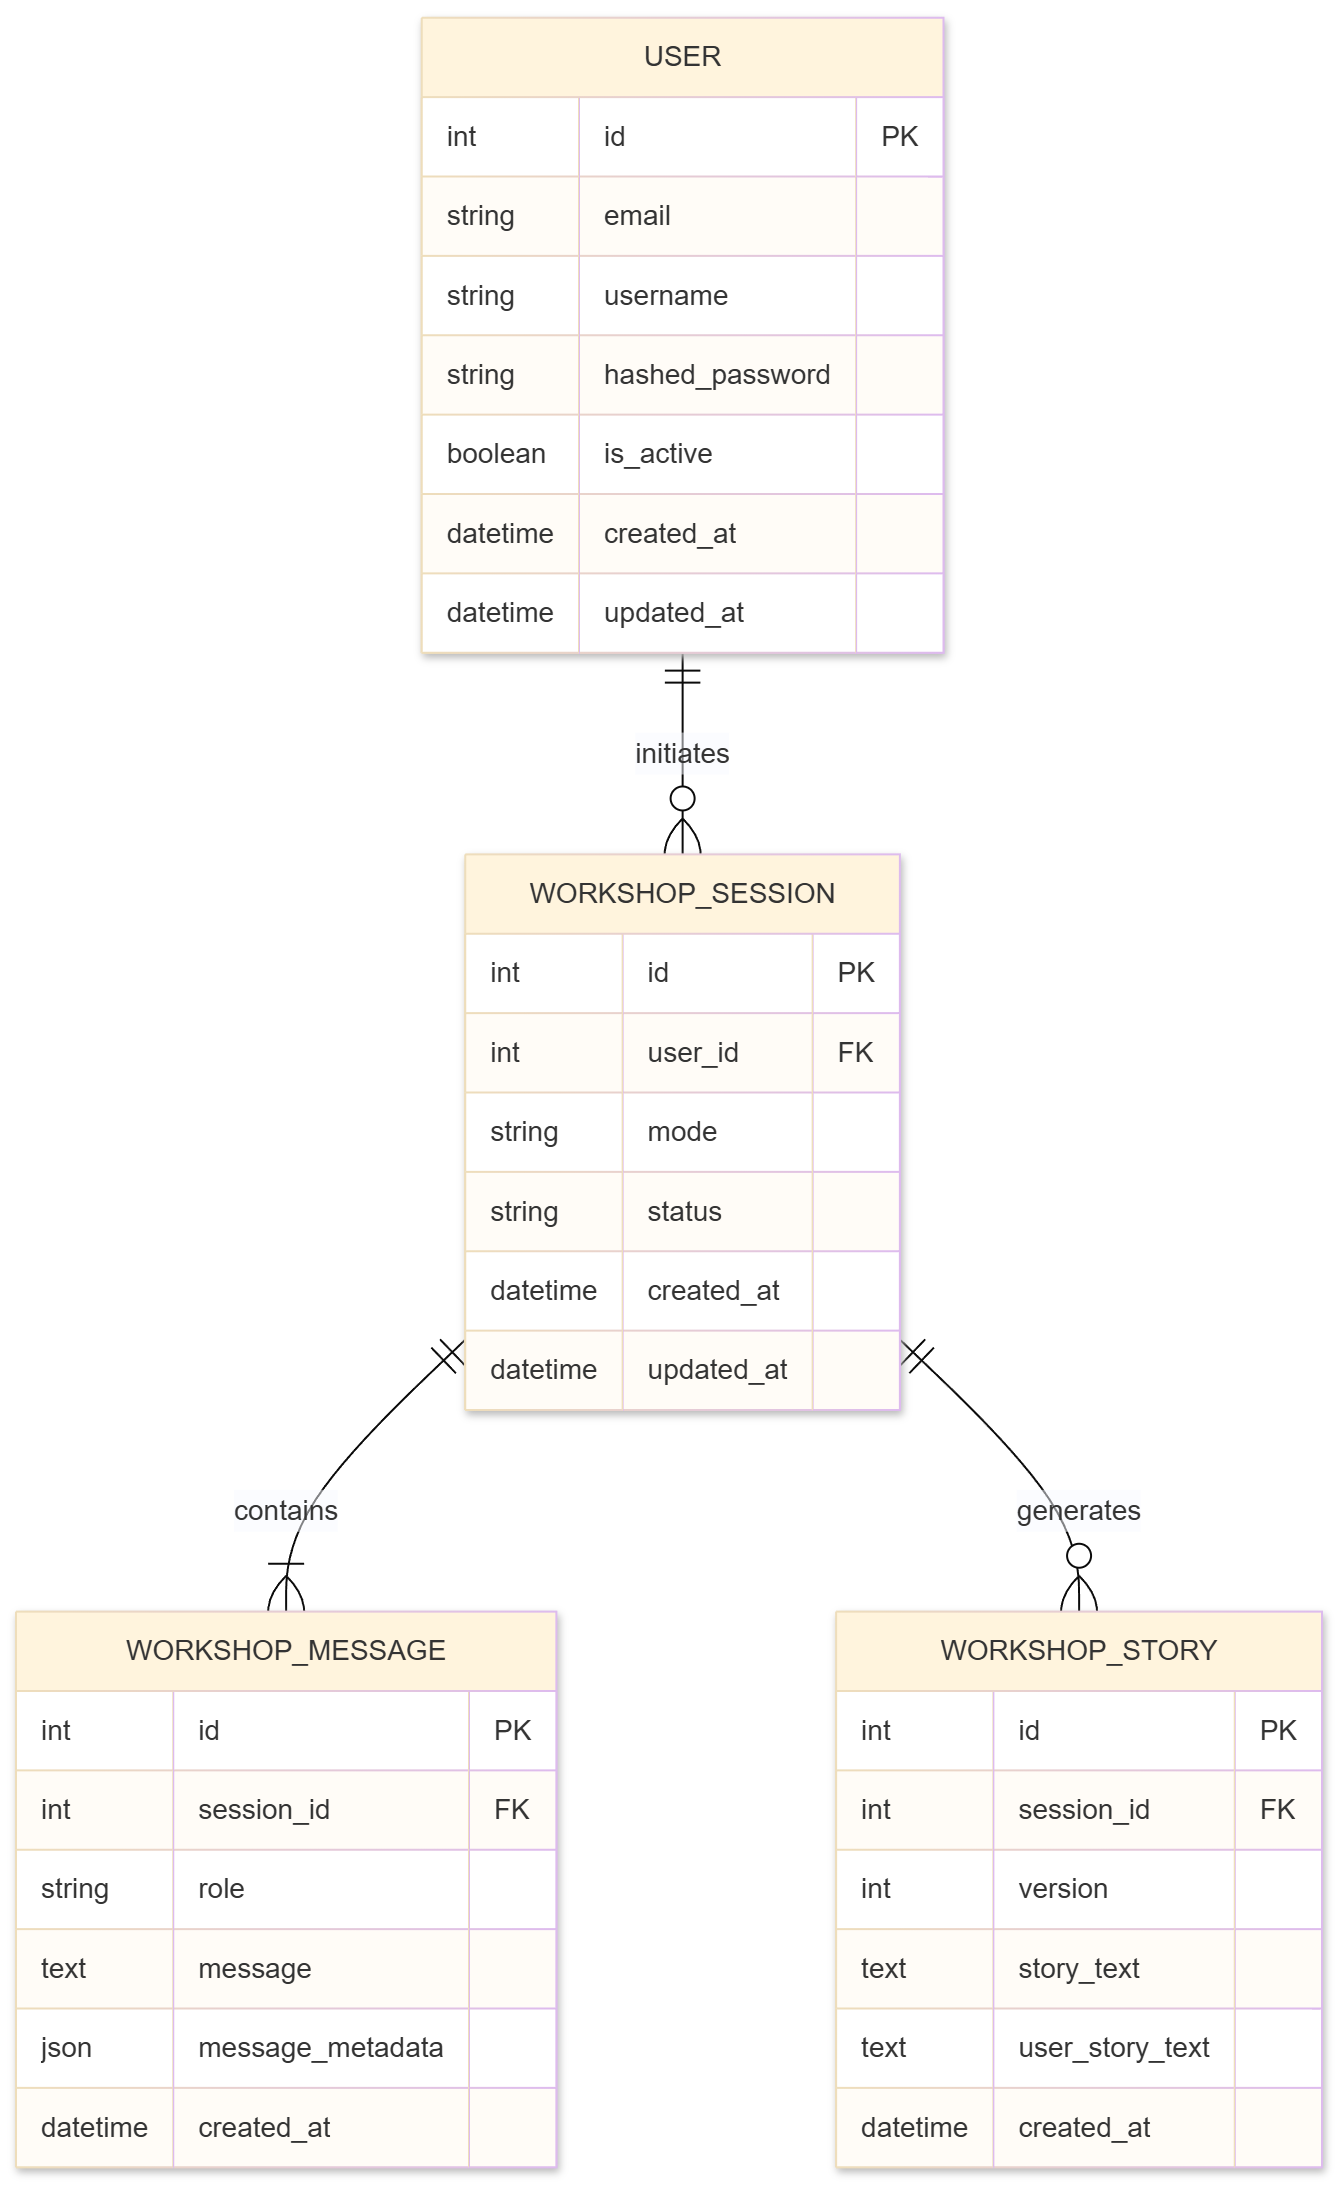
\includegraphics[width=\textwidth]{diagram_images/relational_schema.png}
    \caption{Relational Schema showing database tables and relationships}
    \label{fig:relational_schema}
\end{figure}

\subsection{JSON Story Structure}

Stories are structured in comprehensive JSON format with the following schema:

\begin{itemize}
    \item \textbf{title}: String containing the story title
    \item \textbf{setting}: String describing the story's setting and context
    \item \textbf{characters}: Array of character names
    \item \textbf{scenes}: Array of scene objects, each containing:
    \begin{itemize}
        \item \textbf{scene\_number}: Integer identifier
        \item \textbf{text}: Scene narrative content
        \item \textbf{image\_description}: Description for image generation
        \item \textbf{image\_path}: File system path to generated image
        \item \textbf{image\_url}: Frontend-accessible URL for the image
    \end{itemize}
    \item \textbf{meta}: Optional metadata including genre, style, and generation parameters
\end{itemize}

\section{Domain Model}

The MyAIStorybook domain comprises several core entities that represent the business logic and data structures of the system. The domain model illustrates the relationships between key entities and their attributes.

\begin{figure}[H]
    \centering
    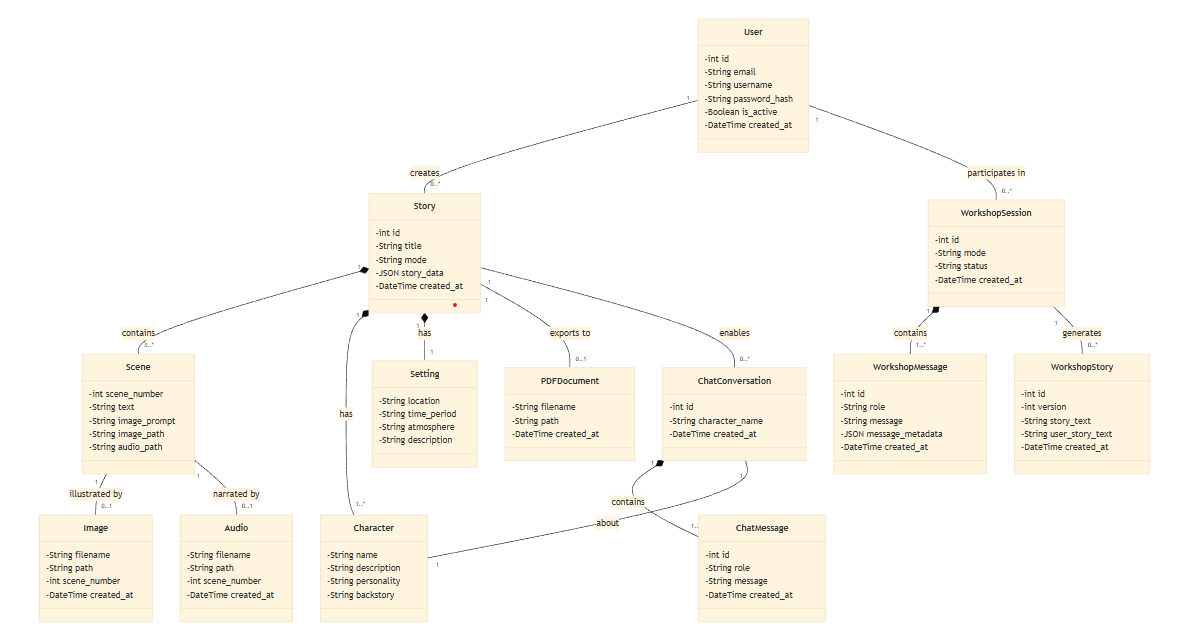
\includegraphics[width=0.9\textwidth]{diagram_images/domain_model.png}
    \caption{Domain Model depicting entities, attributes, and relationships}
    \label{fig:domain_model}
\end{figure}

\textbf{Core Domain Entities:}

\textbf{Story:} Represents a complete generated storybook with metadata, narrative content, and visual elements. Attributes include title, setting, characters (list), scenes (list), and optional metadata.

\textbf{Scene:} Represents an individual page or segment of the story with associated text and optional illustration. Attributes include scene\_number, text, image\_description, and image\_path.

\textbf{Agent (Abstract):} Abstract representation of specialized processing components. Concrete implementations include PromptAgent, WriterAgent, ReviewerAgent, EditorAgent, ImageAgent, DirectorAgent, ChatbotAgent, and EvaluationAgent.

\textbf{User:} Represents authenticated users with attributes for authentication credentials, email, and account metadata. Users can create multiple stories and participate in workshop sessions.

\textbf{WorkshopSession:} Represents interactive idea workshop sessions with mode (improvement/new\_idea), conversation history, and generated story versions.

\section{Design Models}

This section presents detailed design models that capture the system's behavior, structure, and data flow using standard software engineering notations.

\subsection{Class Diagram}

The class diagram illustrates the object-oriented structure of the system, showing classes, their attributes, methods, and relationships.

\begin{figure}[H]
    \centering
    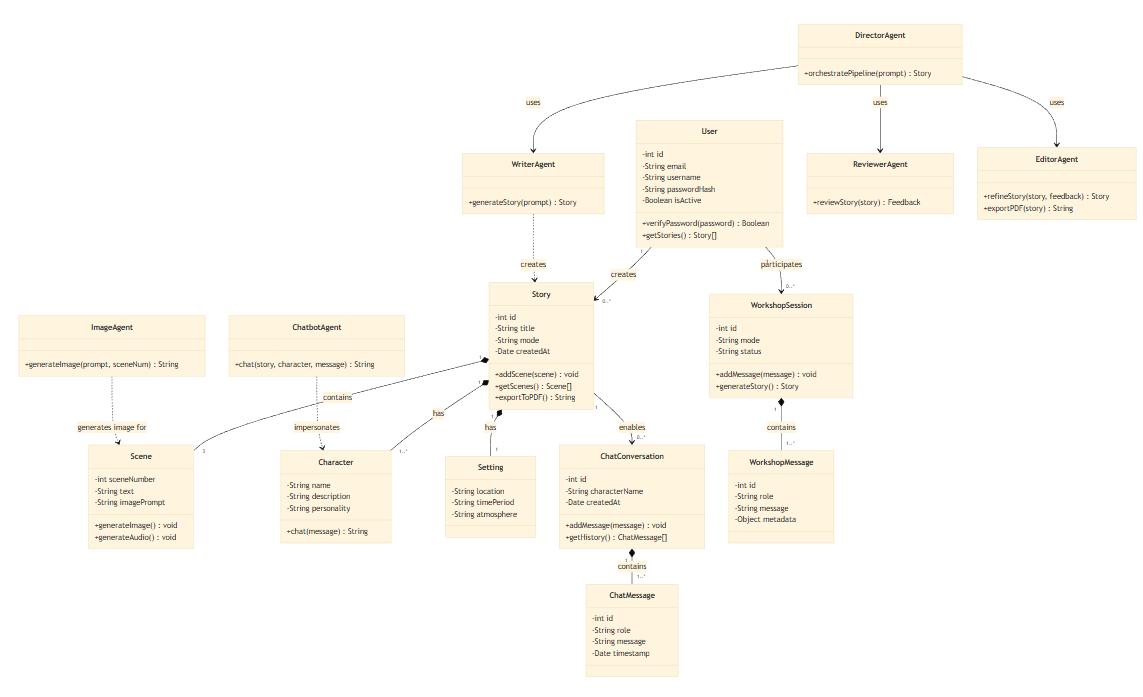
\includegraphics[width=\textwidth]{diagram_images/class_diagram.png}
    \caption{Class Diagram representing the object-oriented design}
    \label{fig:class_diagram}
\end{figure}

\subsection{Data Flow Diagram}

The Data Flow Diagram illustrates how data moves through the system, from user input through various processing stages to final output generation.

\begin{figure}[H]
    \centering
    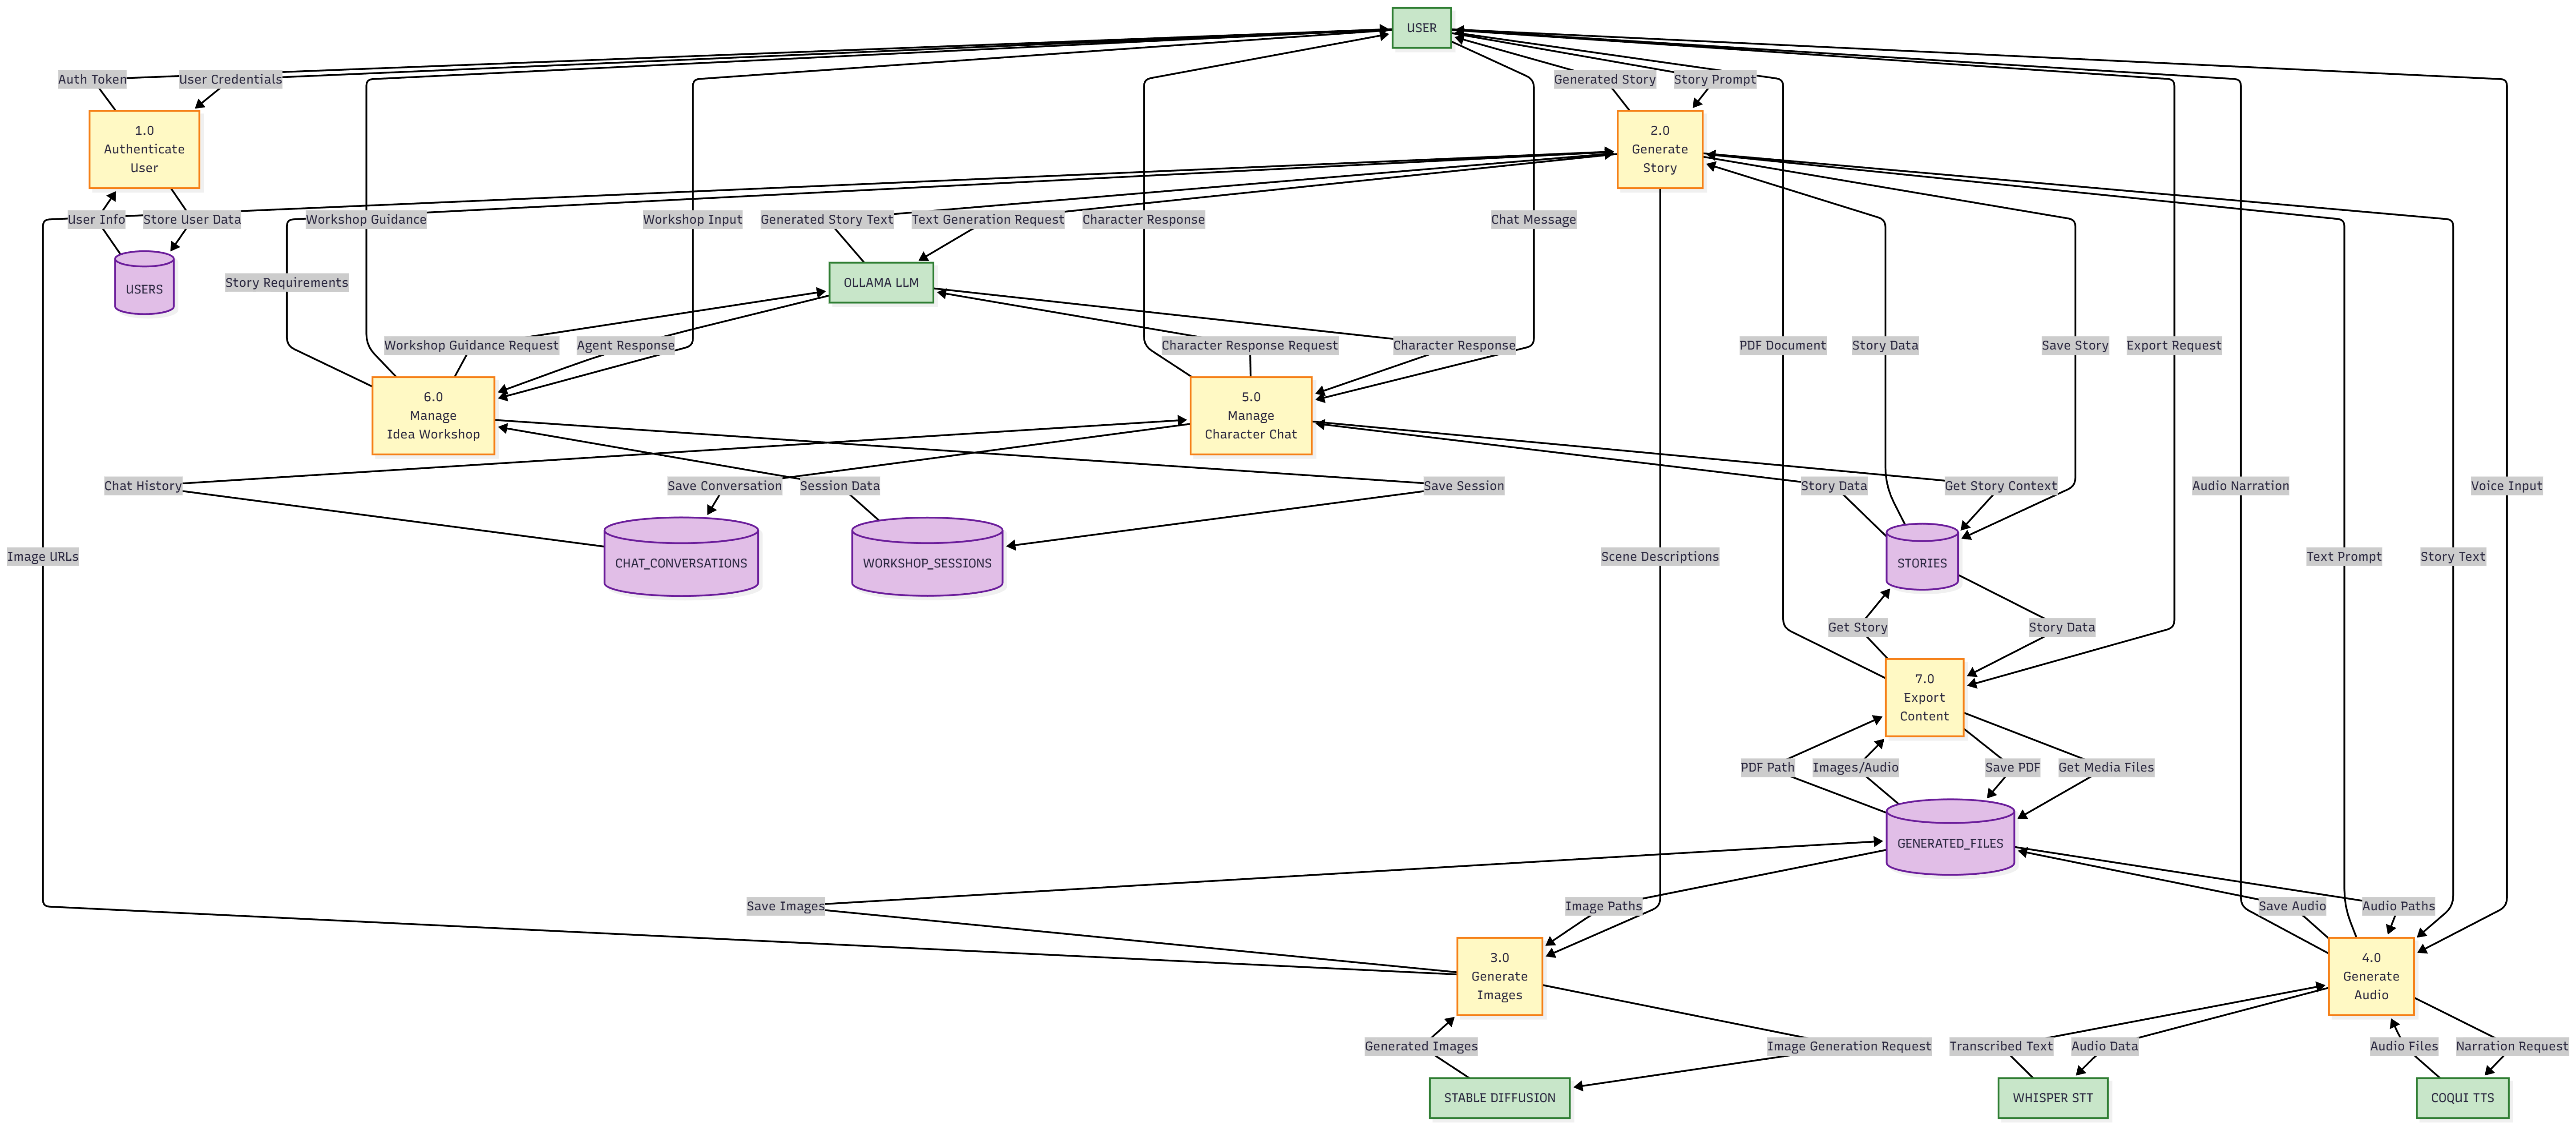
\includegraphics[width=\textwidth]{diagram_images/data_flow_diagram.png}
    \caption{Data Flow Diagram showing information flow through the system}
    \label{fig:data_flow_diagram}
\end{figure}

\subsection{Sequence Diagrams}

Sequence diagrams illustrate the temporal interactions between system components for key use cases.

\subsubsection{Sequence Diagram: Story Generation Workflow}

\begin{figure}[H]
    \centering
    
\includegraphics[width=\textwidth]{diagram_images/sequence_story_generation.png}
    \caption{Sequence Diagram showing complete story generation workflow}
    \label{fig:seq_story_generation}
\end{figure}

This diagram illustrates the complete story generation workflow from user prompt submission through multi-agent processing to final story delivery. The sequence shows interactions between Frontend, FastAPI Backend, PromptAgent, DirectorAgent, WriterAgent, ReviewerAgent, EditorAgent, ImageAgent, and the file system.

\subsubsection{Sequence Diagram: Character Chat Interaction}

\begin{figure}[H]
    \centering
    
\includegraphics[width=0.9\textwidth]{diagram_images/sequence_character_chat.png}
    \caption{Sequence Diagram showing character chat interaction workflow}
    \label{fig:seq_character_chat}
\end{figure}

This diagram demonstrates the character chatbot interaction flow, showing how users engage in conversations with story characters through the ChatbotAgent, which maintains context from the original story.

\subsubsection{Sequence Diagram: Idea Workshop}

\begin{figure}[H]
    \centering
    
\includegraphics[width=\textwidth]{diagram_images/sequence_idea_workshop.png}
    \caption{Sequence Diagram showing idea workshop conversation flow}
    \label{fig:seq_idea_workshop}
\end{figure}

This diagram illustrates the interactive idea workshop workflow where users collaborate with the IdeaWorkshopAgent to refine story concepts through multi-turn conversations before generating the final story.